% Provenance (never printed): cycle 2 "Questionner l'espace et le temps"
% (oceans, seas, continents on the globe) and "Questionner le monde de la
% matiere" (states of water in natural phenomena); see sources/book1/PROVENANCE.md.
% Book 1, grade 2, chapter 1.
\chapter{पृथ्वी पर पानी}\label{ch:g2:water-on-earth}

7 दिसंबर 1972 को चंद्रमा की ओर जा रहे तीन अंतरिक्ष-यात्रियों ने अपना कैमरा
पीछे पृथ्वी की ओर घुमाया। उनकी तस्वीर अब तक खींची गई सबसे मशहूर तस्वीरों
में से एक बन गई। इसे देखो। इसमें सफ़ेद बादल दिखते हैं, थोड़ी-सी भूरी और
पीली ज़मीन, नीचे सफ़ेद बर्फ़ --- और नीला, चारों ओर नीला। अंतरिक्ष से
देखने पर हमारा ग्रह एक नीला ग्रह है।

\begin{omfigure}
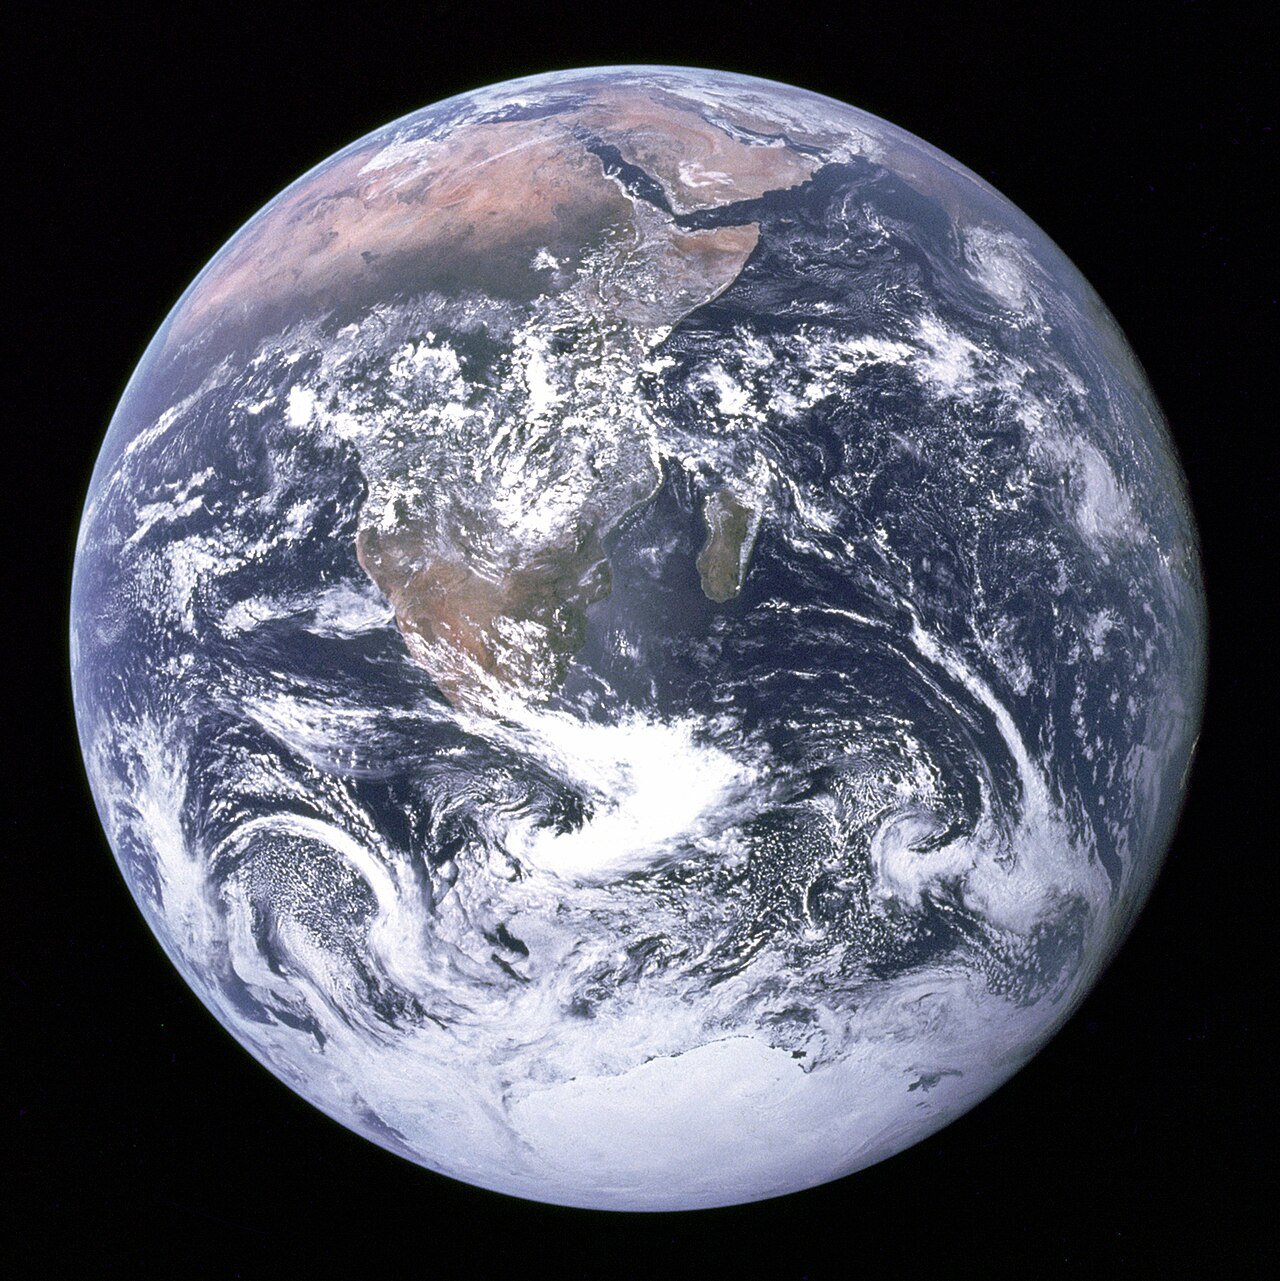
\includegraphics[width=0.5\linewidth]{images/book1/g2-nasa-blue-marble.jpg}

{\small अपोलो~17 के यात्रियों द्वारा 7~दिसंबर 1972 को खींची गई पृथ्वी की
तस्वीर। इसमें अफ़्रीका दिखता है, ऊपर अरब, और नीचे अंटार्कटिका की बर्फ़।
चित्र: नासा (सार्वजनिक डोमेन)।}
\end{omfigure}

\begin{recall}
पानी ठोस (बर्फ़), द्रव, या ऐसी गैस हो सकता है जो हमें दिखती नहीं (जलवाष्प)।
धूप में छोड़ा गया द्रव पानी धीरे-धीरे वाष्प बन जाता है: उसका वाष्पन होता
है। वाष्प ठंडी होने पर फिर से नन्ही बूँदों में बदल जाती है: उसका संघनन
होता है। ये बदलाव तुमने भौतिकी की पुस्तकों में देखे हैं। \omterm{def:g1:landscapes-around-us:landscape}{भूदृश्य} में
पानी \omterm{def:g1:landscapes-around-us:water}{नदियों} में बहता है और \omterm{def:g1:landscapes-around-us:water}{झीलों} में ठहरा रहता है (\cref{ch:g1:landscapes-around-us})।
\end{recall}

\section{नीला ग्रह}

पृथ्वी का ज़्यादातर भाग पानी से ढका है। कल्पना करो कि पृथ्वी की पूरी सतह
को 100 बराबर वर्गों में काट दिया गया है। अगर हम \omterm{def:g2:water-on-earth:ocean}{समुद्र} से ढके हर वर्ग को
नीला रंग दें, तो हम 71 वर्ग रँगेंगे। सिर्फ़ 29 वर्ग ज़मीन हैं।

\begin{omfigure}
\begin{tikzpicture}
  \begin{axis}[hide axis, width=7.2cm, height=7.2cm, xmin=-0.5, xmax=9.5,
      ymin=-0.5, ymax=9.5, axis equal image, scale only axis,
      clip=false]
    \addplot[scatter, only marks, mark=square*, mark size=9.2pt,
      scatter/classes={0={fill=green!45!omLithAlluv, draw=black!40},
                       1={fill=omSea!80!blue, draw=black!40}},
      point meta=explicit symbolic]
      table[x=col, y=row, meta=blue] {figdata/out/grade-2-ocean_fraction-grid.dat};
  \end{axis}
\end{tikzpicture}

{\small अगर पृथ्वी की सतह को 100 बराबर वर्गों में काटा जाए, तो 71 \omterm{def:g2:water-on-earth:ocean}{समुद्र} होंगे
(नीले) और 29 ज़मीन (हरे)। पूरी पृथ्वी की ऊँचाई-निचाई के एक मानचित्र
(NOAA का ETOPO1) से गिना गया।}
\label{fig:g2:water-on-earth:grid}
\end{omfigure}
% ledger: data:etopo1, wss:ocean-cover (71 % computed in figdata/grade-2/ocean_fraction.py)

पृथ्वी के ज़्यादातर भाग को ढकने वाले \omterm{def:g2:water-on-earth:salt-fresh}{खारे पानी} के विशाल फैलावों के नाम हैं।

\begin{definition}[महासागर और समुद्र]\label{def:g2:water-on-earth:ocean}
\emph{महासागर}\index{महासागर} \omterm{def:g2:water-on-earth:salt-fresh}{खारे पानी} के उन बहुत बड़े फैलावों में से एक
है जो पृथ्वी के ज़्यादातर भाग को ढके हुए हैं और महाद्वीपों के बीच फैले हैं।
\emph{समुद्र}\index{समुद्र} \omterm{def:g2:water-on-earth:salt-fresh}{खारे पानी} का इससे छोटा फैलाव है, जो आम तौर पर
किसी महासागर के किनारे होता है और कुछ हद तक ज़मीन से घिरा होता है।
\end{definition}

सारे \omterm{def:g2:water-on-earth:ocean}{महासागर} एक-दूसरे से जुड़े हैं: एक नाव ज़मीन पार किए बिना किसी भी
\omterm{def:g2:water-on-earth:ocean}{महासागर} से किसी भी दूसरे \omterm{def:g2:water-on-earth:ocean}{महासागर} तक जा सकती है। उनके नाम, और ग्लोब पर
वे कहाँ हैं, यह \cref{ch:g3:continents-and-oceans} में है।

\begin{omfigure}
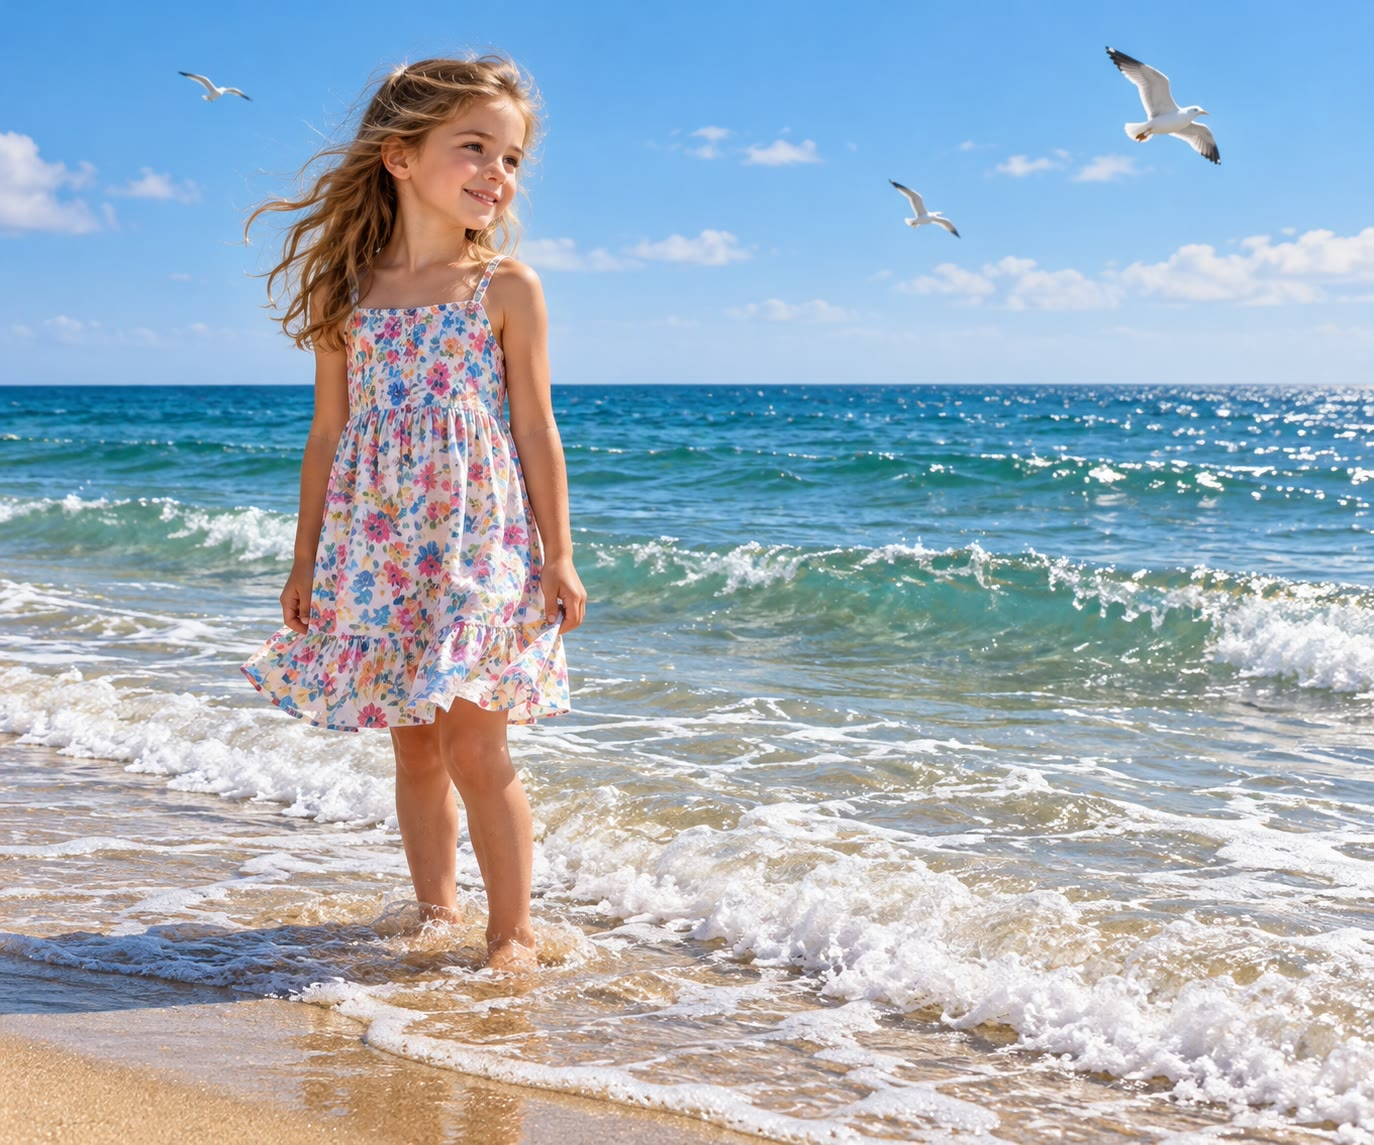
\includegraphics[width=0.62\linewidth]{images/book1/ai/g2-beach-sea.jpg}

{\small \omterm{def:g2:water-on-earth:ocean}{समुद्र} के किनारे। पानी आगे दूर तक फैला है, जहाँ तक आँख देख सकती है
उससे भी कहीं आगे।}
\end{omfigure}

\section{खारा पानी और मीठा पानी}

अगर तैरते समय तुमने कभी \omterm{def:g2:water-on-earth:ocean}{समुद्र} के पानी का घूँट निगला है, तो तुम जानते हो:
उसका स्वाद बहुत नमकीन होता है। \omterm{def:g1:landscapes-around-us:water}{नदियों} और \omterm{def:g1:landscapes-around-us:water}{झीलों} का पानी ऐसा नहीं होता।

\begin{definition}[खारा पानी और मीठा पानी]\label{def:g2:water-on-earth:salt-fresh}
\emph{खारे पानी}\index{खारा पानी} में बहुत-सा नमक घुला होता है: यह
\omterm{def:g2:water-on-earth:ocean}{महासागरों} और \omterm{def:g2:water-on-earth:ocean}{समुद्रों} का पानी है। \emph{मीठे पानी}\index{मीठा पानी} में
बहुत कम नमक होता है: यह बारिश का, ज़्यादातर \omterm{def:g1:landscapes-around-us:water}{नदियों} और \omterm{def:g1:landscapes-around-us:water}{झीलों} का, बर्फ़ और
हिम का, और झरनों का पानी है।
\end{definition}

\begin{example}[समुद्र कितना खारा है?]\label{ex:g2:water-on-earth:salty}
% ledger: nos:salinity
एक किलोग्राम समुद्री पानी --- लगभग एक लीटर --- वाली बोतल में लगभग 35 ग्राम
नमक होता है। अगर हम सारा पानी भाप बनकर उड़ जाने दें, तो नमक तली में सफ़ेद
क्रिस्टलों के रूप में पीछे रह जाता है। \omterm{def:g2:water-on-earth:ocean}{समुद्र} के किनारे नमक के खेतों में
समुद्री नमक इसी तरह बनता है, जहाँ धूप और हवा \omterm{def:g2:water-on-earth:ocean}{समुद्र} के पानी से भरे उथले
कुंडों को धीरे-धीरे सुखा देती हैं।
\end{example}

\begin{omfigure}
\begin{minipage}[b]{0.49\linewidth}\centering
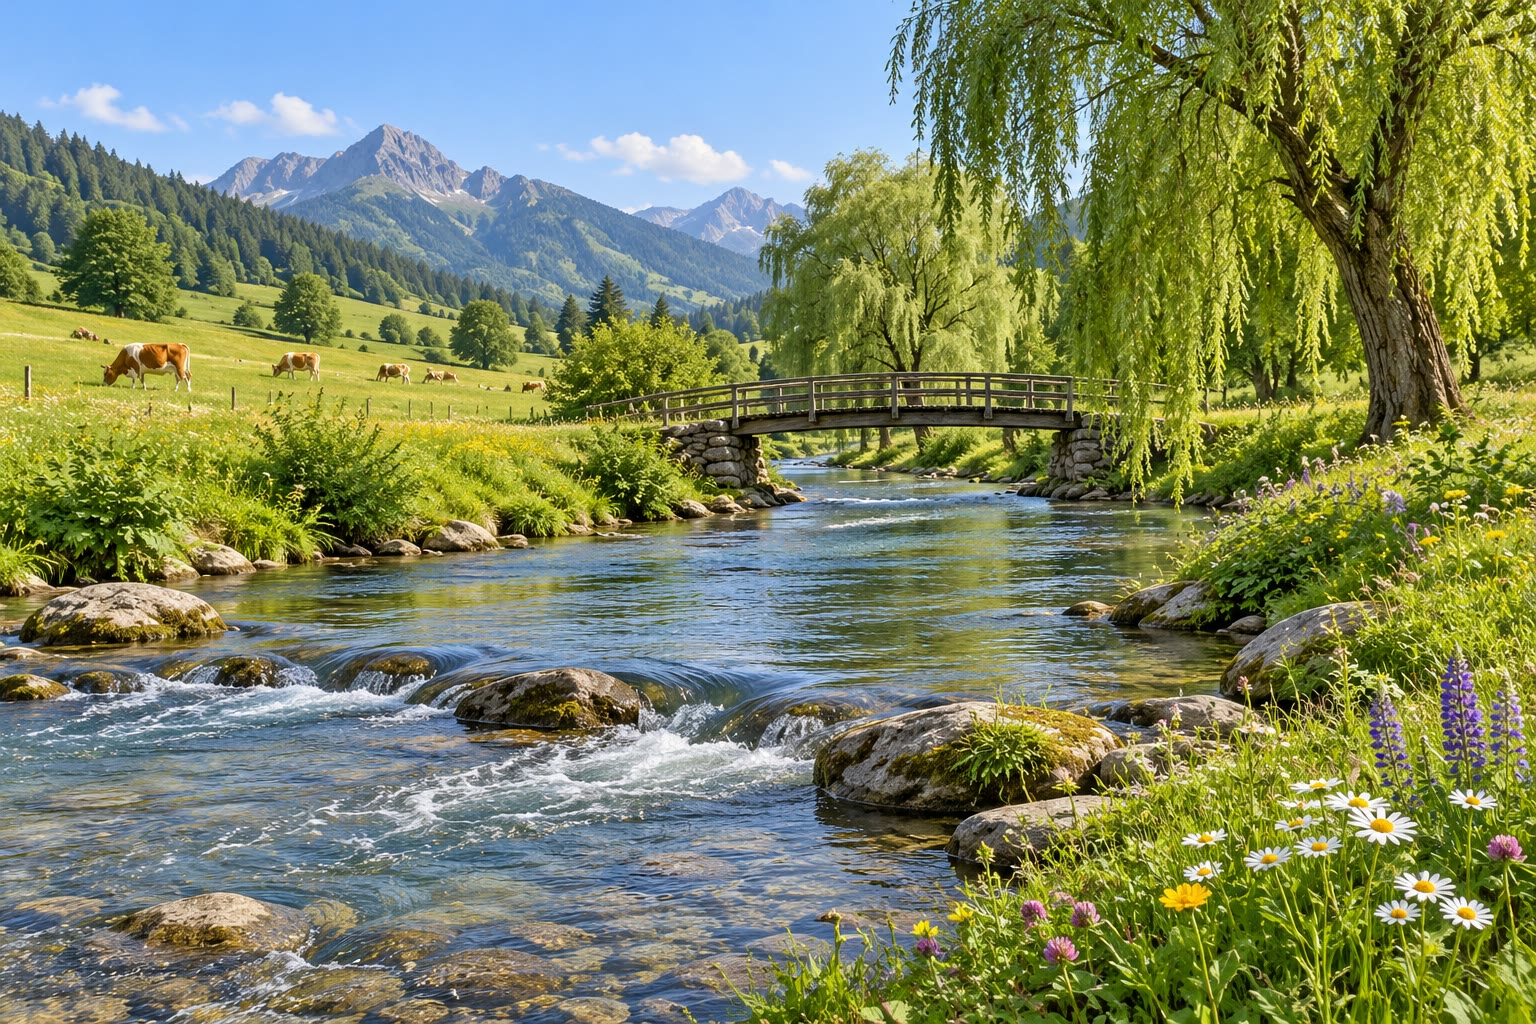
\includegraphics[width=\linewidth]{images/book1/ai/g2-river-meadow.jpg}

{\small \omterm{def:g2:water-on-earth:salt-fresh}{मीठा पानी}: एक \omterm{def:g1:landscapes-around-us:water}{नदी}।}
\end{minipage}\hfill
\begin{minipage}[b]{0.49\linewidth}\centering
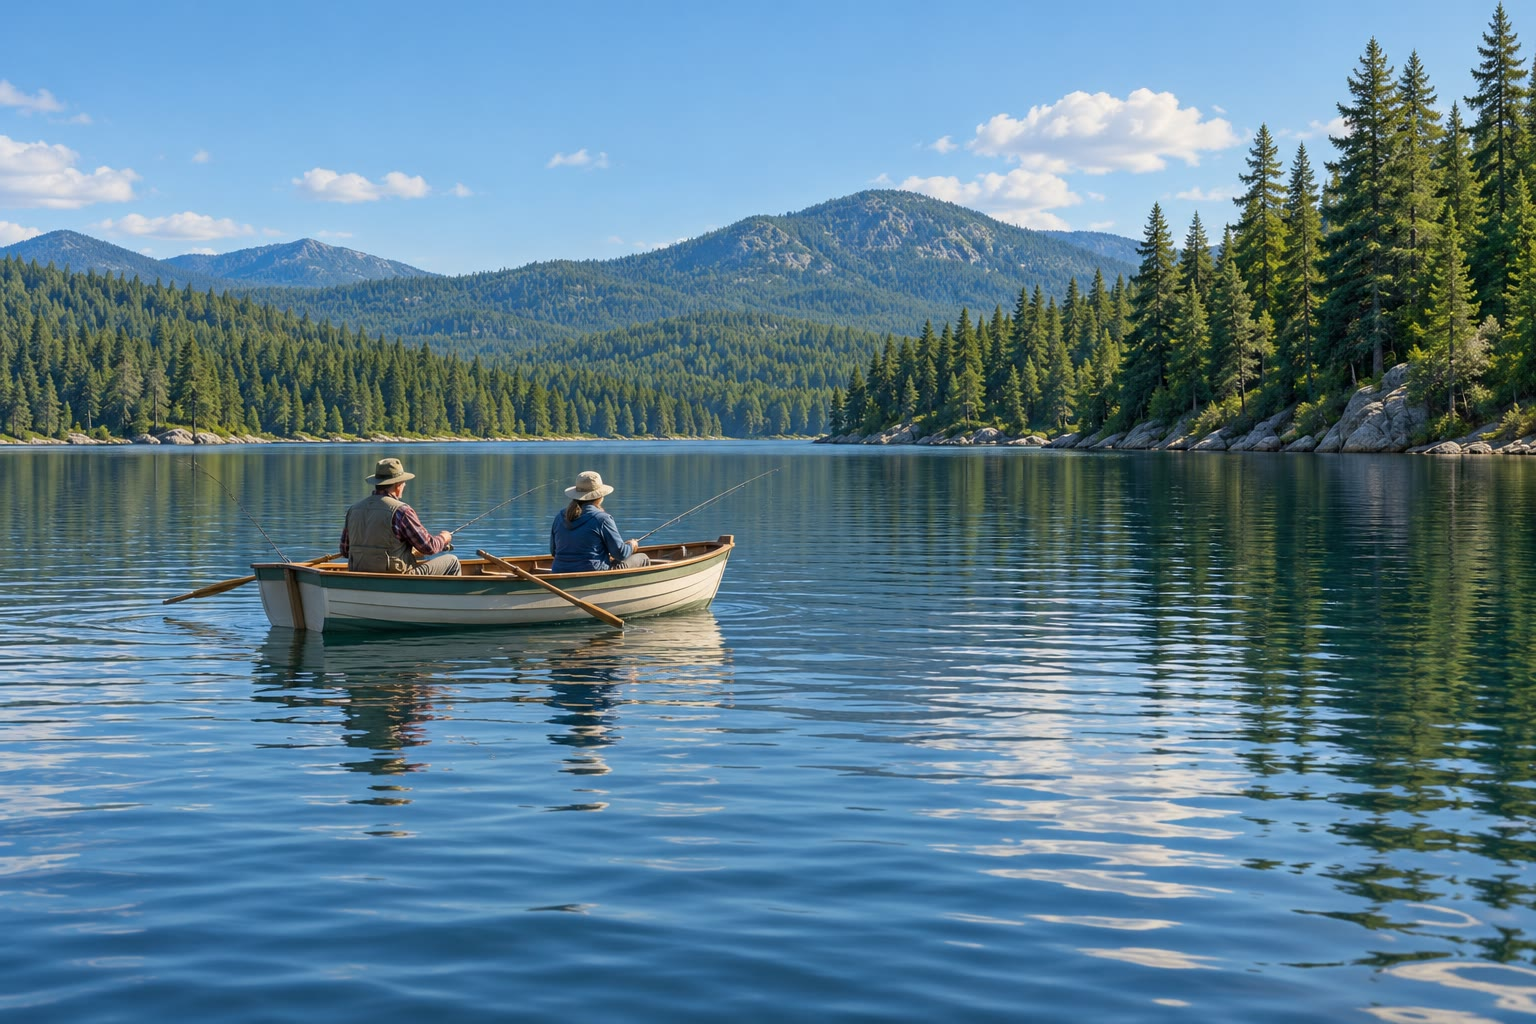
\includegraphics[width=\linewidth]{images/book1/ai/g2-lake-boat.jpg}

{\small \omterm{def:g2:water-on-earth:salt-fresh}{मीठा पानी}: एक \omterm{def:g1:landscapes-around-us:water}{झील}।}
\end{minipage}
\end{omfigure}

\begin{remark}[हम समुद्र का पानी नहीं पी सकते]\label{rem:g2:water-on-earth:drink}
लोग और ज़मीन पर रहने वाले जानवर \omterm{def:g2:water-on-earth:ocean}{समुद्र} का पानी नहीं पी सकते: उसमें बहुत
ज़्यादा नमक होता है, और उसे पीने से शरीर को पानी मिलने की जगह शरीर से पानी
निकल जाता है। \omterm{def:g2:water-on-earth:ocean}{समुद्र} में दूर निकले नाविकों को, चारों ओर पानी होने पर भी,
अपना \omterm{def:g2:water-on-earth:salt-fresh}{मीठा पानी} हमेशा साथ लेकर चलना पड़ा है।
\end{remark}

\section{सारा पानी कहाँ है?}

\omterm{def:g2:water-on-earth:salt-fresh}{मीठा पानी} सिर्फ़ \omterm{def:g1:landscapes-around-us:water}{नदियों} और \omterm{def:g1:landscapes-around-us:water}{झीलों} में ही नहीं है। उसका बहुत-सा भाग जमा हुआ
है: अंटार्कटिका और ग्रीनलैंड की विशाल सफ़ेद बर्फ़ में, और ऊँचे \omterm{def:g1:landscapes-around-us:landform}{पर्वतों} पर।
और उसका बहुत-सा भाग हमारे पैरों के नीचे, ज़मीन में छिपा है, जहाँ वह रेत
के कणों के बीच की नन्ही जगहों और चट्टान की दरारों को भरता है।

\begin{omfigure}
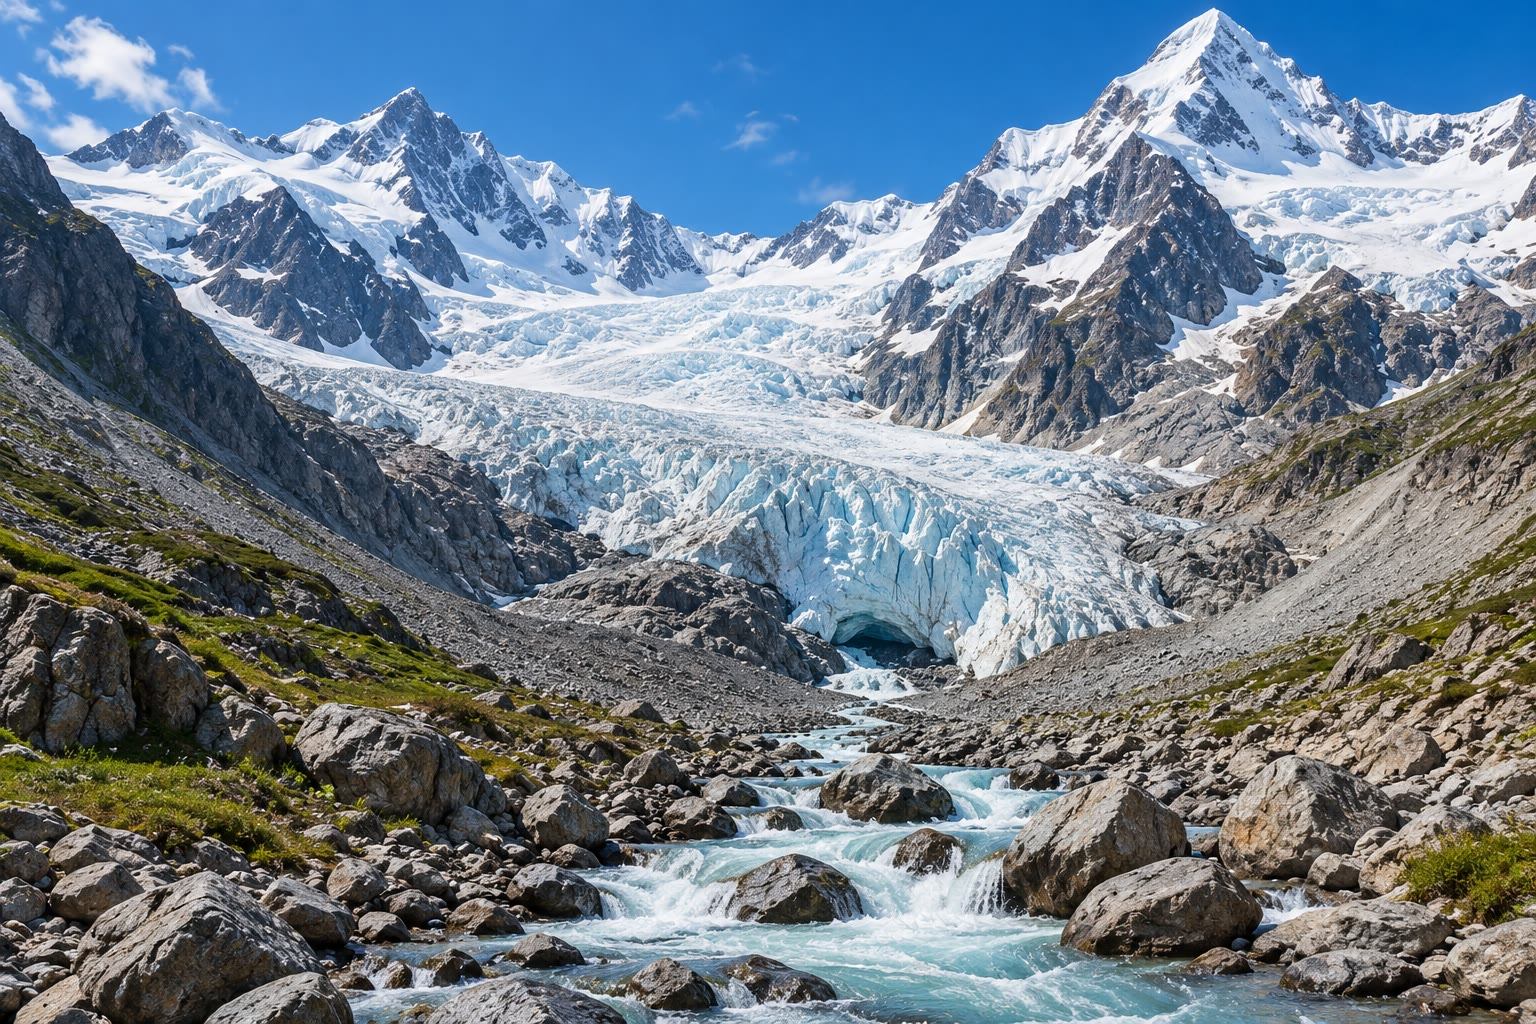
\includegraphics[width=0.62\linewidth]{images/book1/ai/g2-snowy-mountains.jpg}

{\small ऊँचे \omterm{def:g1:landscapes-around-us:landform}{पर्वत} साल भर \omterm{def:g2:water-on-earth:salt-fresh}{मीठे पानी} को हिम और बर्फ़ के रूप में रखते हैं।
गर्मियों में उसका कुछ भाग पिघलकर नालों को पानी देता है।}
\end{omfigure}

कल्पना करो कि हम पृथ्वी का सारा पानी एक ही नाप की 100 बाल्टियों में भर
सकते हैं। हर तरह का पानी कितनी बाल्टियाँ भरेगा?

\begin{omfigure}
\begin{tikzpicture}
  \begin{axis}[hide axis, width=7.2cm, height=7.2cm, xmin=-0.5, xmax=9.5,
      ymin=-0.5, ymax=9.5, axis equal image, scale only axis, clip=false]
    \addplot[scatter, only marks, mark=*, mark size=8pt,
      scatter/classes={0={fill=omSea!80!blue, draw=black!40},
                       1={fill=white, draw=black!60},
                       2={fill=brown!55, draw=black!40}},
      point meta=explicit symbolic]
      table[x=col, y=row, meta=kind] {figdata/out/grade-2-water_shares.dat};
  \end{axis}
  \begin{scope}[shift={(7.9,5.6)}, font=\small]
    \fill[omSea!80!blue, draw=black!40] (0,0) circle (0.2);
    \node[anchor=west] at (0.35,0) {महासागरों का खारा पानी: 96 बाल्टियाँ};
    \fill[white, draw=black!60] (0,-0.7) circle (0.2);
    \node[anchor=west] at (0.35,-0.7) {बर्फ़ और हिम: 2 बाल्टियाँ};
    \fill[brown!55, draw=black!40] (0,-1.4) circle (0.2);
    \node[anchor=west] at (0.35,-1.4) {ज़मीन के नीचे का पानी: 2 बाल्टियाँ};
  \end{scope}
\end{tikzpicture}

{\small पृथ्वी का सारा पानी 100 बाल्टियों में। \omterm{def:g1:landscapes-around-us:water}{नदियाँ}, \omterm{def:g1:landscapes-around-us:water}{झीलें}, बादल और सारे
सजीवों का पानी मिलकर भी एक बाल्टी नहीं भरेंगे। आँकड़े अमेरिकी भूवैज्ञानिक
सर्वेक्षण (USGS) से।}
\label{fig:g2:water-on-earth:buckets}
\end{omfigure}
% ledger: wss:water-shares (rounded to 100 buckets in figdata/grade-2/water_shares.py)

\begin{proposition}[पृथ्वी का ज़्यादातर पानी खारा है]\label{prop:g2:water-on-earth:most-salty}
% ledger: wss:water-shares
पृथ्वी के सारे पानी की 100 बाल्टियों में से 96 \omterm{def:g2:water-on-earth:ocean}{महासागरों} का \omterm{def:g2:water-on-earth:salt-fresh}{खारा पानी} हैं।
जो \omterm{def:g2:water-on-earth:salt-fresh}{मीठा पानी} हम पीते हैं, वह सारे पानी का बहुत ही छोटा भाग है: उसका
ज़्यादातर भाग बर्फ़ में जमा है, या ज़मीन के नीचे छिपा है।
\end{proposition}

\section{बारिश का पानी कहाँ जाता है?}

जब बारिश होती है, तो पानी वहीं नहीं रुकता जहाँ वह गिरता है। बौछार के बाद
स्कूल के आँगन को देखो: कुछ पानी ज़मीन पर बहकर नालियों में चला जाता है,
कुछ क्यारियों की मिट्टी में रिस जाता है, और धूप लौटने पर डबरे धीरे-धीरे
ग़ायब हो जाते हैं।

\begin{omfigure}
\begin{tikzpicture}[x=1cm, y=1cm, font=\small]
  % sky, sea, land
  \fill[ocBlue!6] (0,0) rectangle (12,5.6);
  \fill[omSea] (8.6,0) rectangle (12,0.9);
  \fill[green!30!omLithAlluv] (0,0) -- (0,2.4) .. controls (2,2.6) and (3,2.0) .. (4.5,1.6)
     .. controls (6,1.2) and (7.5,1.0) .. (8.6,0.9) -- (8.6,0) -- cycle;
  % ground below the surface
  \fill[brown!25] (0,0) rectangle (8.6,0.6);
  % river
  \draw[omSea!70!blue, line width=2.4pt] (1.6,2.45) .. controls (3.5,2.0) and (6,1.15) .. (8.6,0.95);
  % cloud and rain
  \pic at (2.2,4.0) {puffycloud};
  \foreach \x in {1.4,1.8,2.2,2.6,3.0}
    \draw[omWxRain, line width=0.8pt] (\x,3.7) -- (\x-0.15,3.1);
  \pic at (9.6,4.3) {puffycloud};
  % arrows
  \draw[omWxRain, line width=1.1pt, -{Stealth[length=2.5mm]}] (3.3,2.15) -- (3.3,0.6);
  \node[anchor=west, align=left, font=\scriptsize] at (3.4,1.0) {कुछ ज़मीन\\में रिसता है};
  \draw[omWxRain, line width=1.1pt, -{Stealth[length=2.5mm]}] (5.4,1.55) -- (7.6,1.15);
  \node[align=center, font=\scriptsize] at (6.2,2.05) {कुछ नदी में बहता है,\\और नदी समुद्र तक};
  \draw[black!50, line width=1.1pt, densely dashed, -{Stealth[length=2.5mm]}] (10.2,1.1) .. controls (10.4,2.4) and (10.1,3.2) .. (9.8,3.85);
  \node[align=left, anchor=west, font=\scriptsize] at (10.45,2.4) {पानी का\\वाष्पन};
  \draw[black!50, line width=1.1pt, densely dashed, -{Stealth[length=2.5mm]}] (8.45,4.35) -- (3.6,4.3);
  \node[font=\scriptsize, above] at (6.0,4.35) {हवा बादलों को ले जाती है};
  \node[font=\scriptsize] at (10.4,0.45) {समुद्र};
  \node[font=\scriptsize, anchor=west] at (0.2,3.25) {बारिश};
\end{tikzpicture}

{\small बारिश का पानी कहाँ जाता है। \omterm{def:g2:water-on-earth:ocean}{समुद्र} और ज़मीन से वाष्प बनकर ऊपर उठने
वाला पानी नए बादल बनाता है, और बादल नई बारिश लाते हैं।}
\label{fig:g2:water-on-earth:rain}
\end{omfigure}

\begin{method}[बारिश की एक बूँद का पीछा करना]\label{met:g2:water-on-earth:drop}
बारिश की एक बूँद का पीछा करने के लिए बारी-बारी से तीन सवाल पूछो:
\begin{enumerate}
  \item वह कहाँ गिरती है: \omterm{def:g2:water-on-earth:ocean}{समुद्र} पर, छत पर, मिट्टी पर, किसी \omterm{def:g1:landscapes-around-us:landform}{पर्वत} पर?
  \item वह ज़मीन में रिस जाती है, सतह पर बह जाती है, या जमकर बर्फ़ बन
        जाती है?
  \item वह आगे कहाँ जाती है: \omterm{def:g1:landscapes-around-us:water}{नदी} में, \omterm{def:g1:landscapes-around-us:water}{झील} में, \omterm{def:g2:water-on-earth:ocean}{समुद्र} में, ज़मीन में, या
        वापस हवा में?
\end{enumerate}
आख़िर में हर बूँद \omterm{def:g2:water-on-earth:ocean}{समुद्र} में या हवा में लौट आती है, और यात्रा फिर से शुरू
हो जाती है।
\end{method}

\begin{example}[पर्वत पर एक बूँद]\label{ex:g2:water-on-earth:mountain}
बारिश की एक बूँद सर्दियों में किसी ऊँचे \omterm{def:g1:landscapes-around-us:landform}{पर्वत} पर हिम बनकर गिरती है। वह
वहाँ जमी रहती है, गर्मियों के गरम दिनों तक। फिर वह पिघलती है, बहकर
\omterm{def:g1:landscapes-around-us:landform}{पहाड़ी} नाले में जाती है, एक \omterm{def:g1:landscapes-around-us:water}{नदी} से मिलती है, और \omterm{def:g1:landscapes-around-us:water}{नदी} उसे \omterm{def:g2:water-on-earth:ocean}{समुद्र} तक ले
जाती है। किसी धूप वाले दिन बूँद का \omterm{def:g2:water-on-earth:ocean}{समुद्र} से वाष्पन होता है और वह ऊपर
हवा में उठती है, जहाँ वह एक नए बादल का हिस्सा बन जाती है।
\end{example}

\section{अभ्यास}

\begin{exercise}[$\star$]\label{exo:g2:water-on-earth:1}
\omterm{def:g2:water-on-earth:salt-fresh}{खारा पानी} या \omterm{def:g2:water-on-earth:salt-fresh}{मीठा पानी}? \omterm{def:g2:water-on-earth:ocean}{समुद्र}; \omterm{def:g1:landscapes-around-us:water}{नदी}; बारिश; \omterm{def:g1:landscapes-around-us:landform}{पर्वतों} में एक \omterm{def:g1:landscapes-around-us:water}{झील}; \omterm{def:g2:water-on-earth:ocean}{महासागर};
\omterm{def:g1:landscapes-around-us:landform}{पर्वत} पर की बर्फ़।
\end{exercise}

\begin{exercise}[$\star$]\label{exo:g2:water-on-earth:2}
हम पृथ्वी को ``नीला ग्रह'' क्यों कहते हैं?
\end{exercise}

\begin{exercise}[$\star$]\label{exo:g2:water-on-earth:3}
100 वर्गों वाले जाल में 71 वर्ग नीले हैं। कितने वर्ग ज़मीन हैं?
\end{exercise}

\begin{exercise}[$\star$]\label{exo:g2:water-on-earth:4}
कौन बड़ा है, \omterm{def:g2:water-on-earth:ocean}{महासागर} या \omterm{def:g2:water-on-earth:ocean}{समुद्र}?
\end{exercise}

\begin{exercise}[$\star$]\label{exo:g2:water-on-earth:5}
क्या \omterm{def:g2:water-on-earth:ocean}{महासागर} के बीच में कोई नाविक अपनी नाव के चारों ओर का पानी पी सकता है?
क्यों?
\end{exercise}

\begin{exercise}[$\star$]\label{exo:g2:water-on-earth:6}
तीन ऐसी जगहों के नाम बताओ जहाँ \omterm{def:g2:water-on-earth:salt-fresh}{मीठा पानी} मिलता है।
\end{exercise}

\begin{exercise}[$\star\star$]\label{exo:g2:water-on-earth:7}
100 बाल्टियों वाले चित्र में कितनी बाल्टियाँ \omterm{def:g2:water-on-earth:salt-fresh}{खारा पानी} हैं? कितनी \omterm{def:g2:water-on-earth:salt-fresh}{मीठा
पानी} हैं (बर्फ़ और ज़मीन के नीचे का पानी मिलाकर)?
\end{exercise}

\begin{exercise}[$\star\star$]\label{exo:g2:water-on-earth:8}
इन्हें क्रम में लगाओ, सबसे ज़्यादा पानी रखने वाले से सबसे कम पानी रखने वाले
तक: \omterm{def:g1:landscapes-around-us:water}{नदियाँ}; \omterm{def:g2:water-on-earth:ocean}{महासागर}; बर्फ़ और हिम।
\end{exercise}

\begin{exercise}[$\star\star$]\label{exo:g2:water-on-earth:9}
एक खेत पर बारिश होती है। पानी के साथ हो सकने वाली दो बातें बताओ।
\end{exercise}

\begin{exercise}[$\star\star$]\label{exo:g2:water-on-earth:10}
\omterm{def:g2:water-on-earth:ocean}{समुद्र} के पानी से भरा एक तसला कई दिनों तक धूप में छोड़ दिया जाता है, जब
तक पानी ख़त्म न हो जाए। तसले की तली में क्या बचता है? पानी कहाँ गया?
\end{exercise}

\begin{exercise}[$\star\star$]\label{exo:g2:water-on-earth:11}
स्कूल की छत पर गिरने वाली बारिश की एक बूँद की यात्रा बताओ, तब तक की जब
तक वह फिर से किसी बादल में न पहुँच जाए।
\end{exercise}
